\chapter{Implementierungsplan}
\label{ch:implplan}
Um einen Implementierungsplan aufzustellen, wurde das Projekt zuerst anhand der einzelnen Plugins/Pakete aufgeteilt. Danach wurden die Plugins/Pakete noch feiner unterteilt und es wurde versucht einzelne, möglichst voneinander unabhängige, Aufgaben zu finden. Der nötige Arbeitsaufwand zum Bearbeiten der einzelnen Aufgaben wurden von allen Projektmitgliedern abgeschätzt und der Mittelwert als geplante Bearbeitungsdauer festgesetzt. Anhand von den bestehenden Abhängigkeiten der Aufgaben untereinander und der vorausgesetzten wöchentlichen Arbeitsleistung, wurden die Aufgaben auf die einzelnen Wochen und Personen verteilt. \\
\begin{figure}[!htbp]
	\centering
	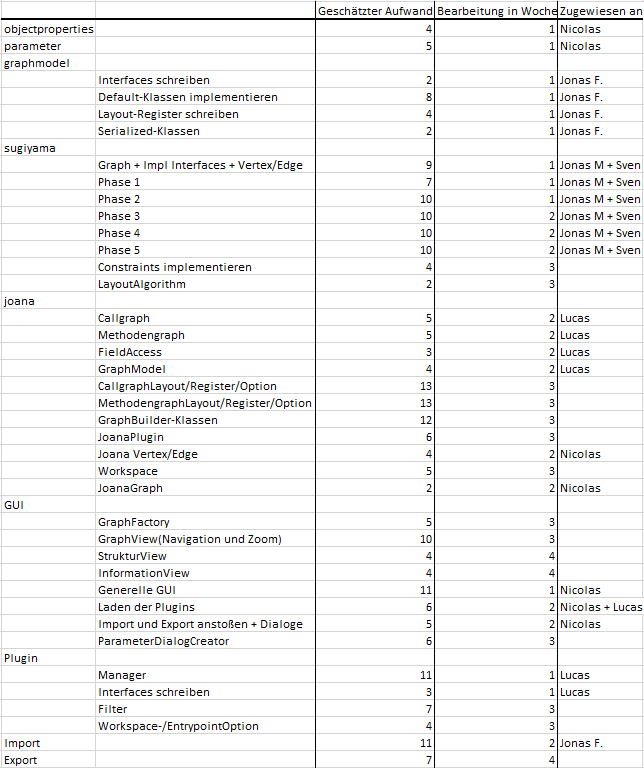
\includegraphics[width=300pt]{week_zero_table.PNG}
	\caption{Erster Implementierungsplan}
	\label{fig:week_zero_table}
\end{figure}

\newpage

\section{Woche 1}
In der ersten Woche wurde der zuerst erstellte Implementierungsplan jedoch komplett überarbeitet. Dies war nötig da im ersten Plan viele Abhängigkeiten zwischen den Aufgaben nicht berücksichtigt wurden. Zum Beispiel hing das restliche Projekt komplett von der Fertigstellung des Sugiyama ab und hätte ohne diesen nicht getestet werden können. Um dieses Problem zu lösen, wurden vorläufige Mockups für die einzelnen Phasen eingeplant. Die anderen Aufgaben wurden zusätzlich in der Abarbeitungsreihenfolge umsortiert, verfeinert und für die ersten zwei Wochen bereits einzelnen Personen zugewiesen. Außerdem wurde eine Excel Tabelle mit dem bereits existierenden Plan erstellt und durch eine Fortschrittsspalte erweitert. In der Fortschrittspalte sollten die Entwickler den prozentualen Fortschritt an den ihnen zugeteilten Aufgaben eintragen. Dadurch konnte ein Fortschrittsdiagram erstellt werden, welchen den aktuellen Soll- und Ist-Zustand des gesamten Projekt visualisiert.\\
\\
Zusätzlich zur Änderung des Plans wurde eine grobe Projektstruktur in Gradle aufgebaut und die bereits im Entwurf erstellte Interfaces in das Projekt überführt. Um die Gradle Projektkonfiguration zu testen wurde eine grobe GUI implementiert und mit der Implementierung der Allgemein genutzten Klassen aus dem Paket "graphmodel"  begonnen.
\begin{figure}[!htbp]
	\centering
	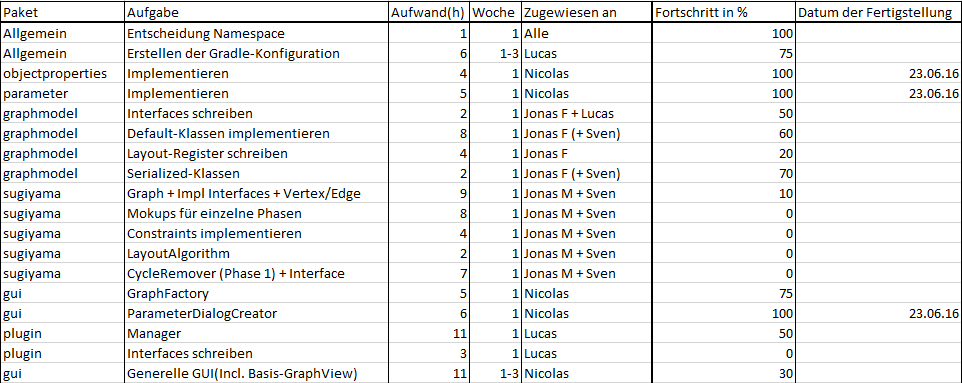
\includegraphics[width=380pt]{week_one_table.PNG}
	\caption{Überarbeiteter Plan nach Woche 1 mit Fortschritt}
	\label{fig:week_one_table}
\end{figure}
\subsection{Verzögerungen}
Wie man in \ref{fig:week_one_diagram} sehen kann, hing das Projekt nach der ersten Woche bereits ca. 35 Stunden hinter dem geplanten Zustand hinterher.
Dies lag neben der Tatsache, dass die erste Hälfte der Woche aufgrund von Erschöpfung aus der Entwurfsphase, weniger gearbeitet wurde, als auch daran, dass das Team, welches für die Implementierung des Sugiyama-Layoutalgorithmus eingeteilt wurde, relativ schnell auf konzeptionelle Probleme mit dem im Entwurf definierten Aufbau des SugiyamaGraphen und dessen Kanten/Knoten stieß(siehe \ref{sec:change_sugiyama}).
\begin{figure}[!htbp]
	\centering
	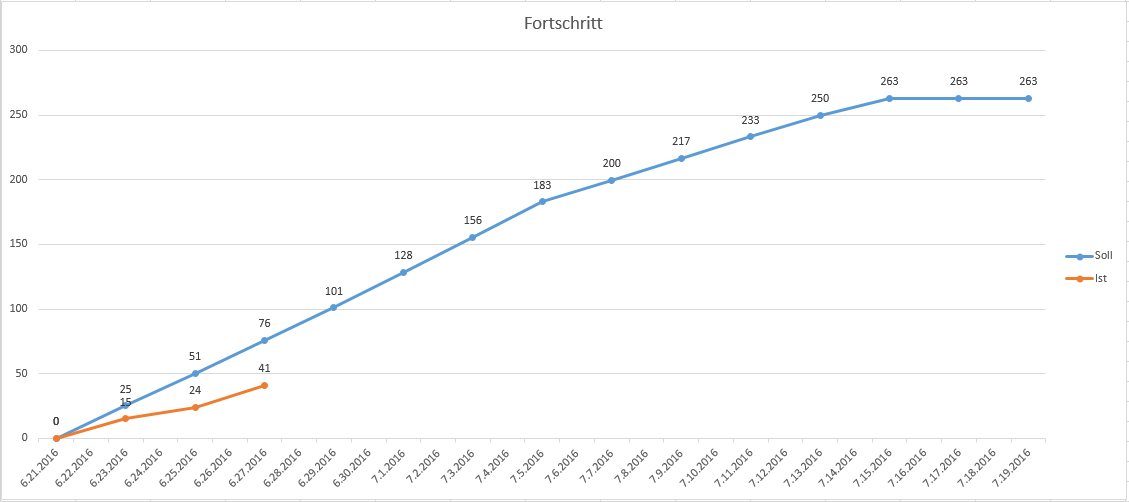
\includegraphics[width=380pt]{resourcen/week_one_diagram.PNG}
	\caption{Fortschrittsdiagramm nach Woche 1}
	\label{fig:week_one_diagram}
\end{figure}

\newpage

\section{Woche 2}
Das Ziel der Woche 2 war es, einen Graphen zu importieren und diesen, mithilfe von Mockups im Sugiyama-Algorithmus, in der Graphansicht anzuzeigen.
Dazu wurde besonders auf die zeitnahe Fertigstellung des Imports und auf die grobe Implementierung des JOANA-Graph-Plugins mit allen dazugehörigen Klassen geachtet. Zudem wurde auch in den einzelnen Phasen des Sugiyama-Algorithmus große Fortschritte gemacht und einige wurden sogar abgeschlossen. Dadurch entstand der, wie in \ref{fig:week_two_diagram} zu sehen ist, sprunghafte Anstieg des Fortschritts, welcher fast den Soll-Wert erreichte. 
\begin{figure}[!htbp]
	\centering
	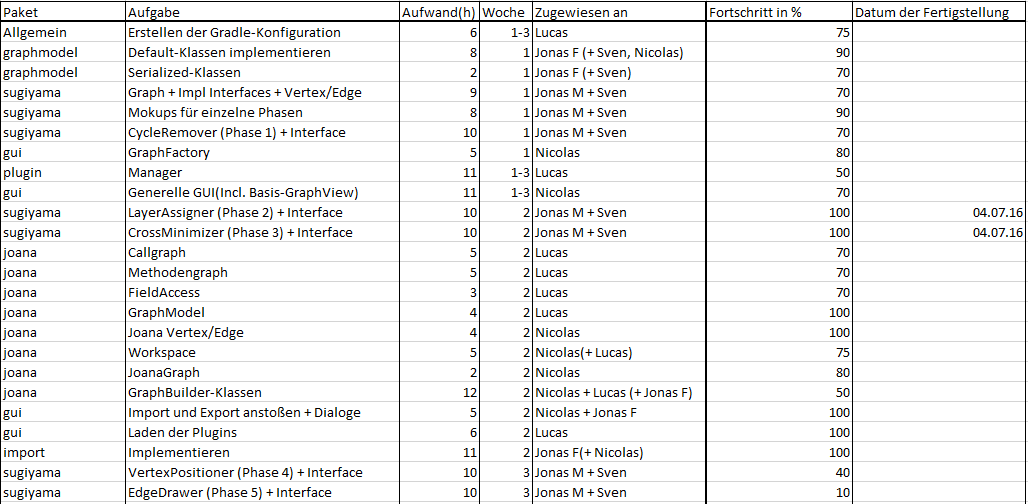
\includegraphics[width=380pt]{week_two_table.PNG}
	\caption{Implementierungsplan nach Woche 1 und 2}
	\label{fig:week_two_table}
\end{figure}
\subsection{Verzögerungen}
\label{sec:delay_week2}
Aufgrund der im Entwurf definierten Generics im GraphModel entstanden häufig sehr unschöne Stellen im Code und Inkompatibilitäten. Diese zu reparieren oder funktionsfähig zu machen war häufig der Grund für mehr oder weniger unschöne Workarounds, die teilweise viel Arbeit in Anspruch nahmen. Deshalb wurde für die folgende Woche ein großes Refactoring angesetzt, welches die Generic-Struktur im GraphModel stark vereinfachen soll.
\begin{figure}[!htbp]
	\centering
	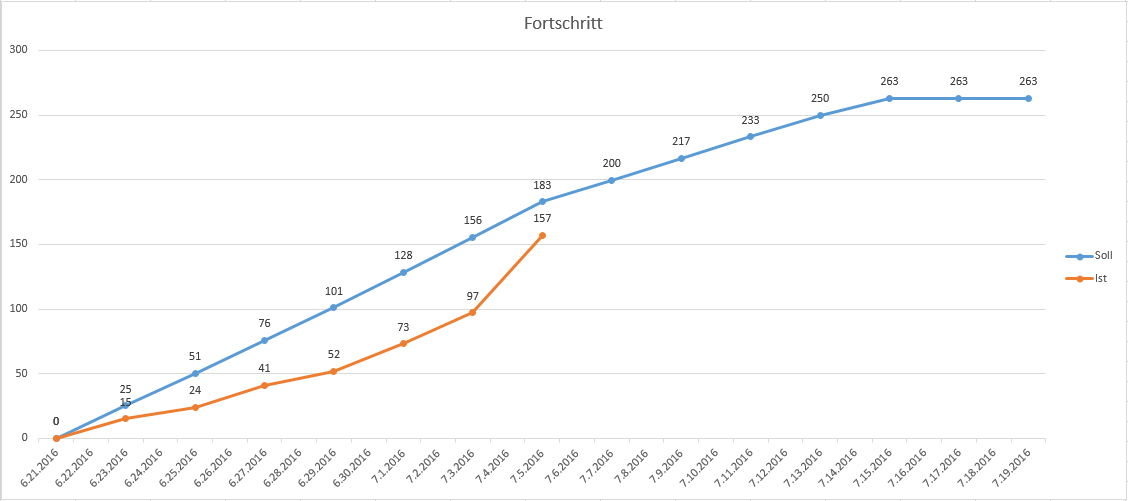
\includegraphics[width=380pt]{resourcen/week_two_diagram.PNG}
	\caption{Fortschrittsdiagramm nach Woche 2}
	\label{fig:week_two_diagram}
\end{figure}

\newpage

\section{Woche 3}
Da in Woche 3 die Oberfläche benutzbar war und man Graphen importieren und anzeigen konnte wurde neben dem in \ref{sec:delay_week2} beschriebenen Refactoring, viele Bugfixes und Verbesserungen vorgenommen, die ohne eine Anzeige nicht sichtbar waren. Genau deshalb wurden in \ref{fig:week_three_table} zwar weniger Aufgaben vollständig abgeschlossen, dafür bei vielen aber ein deutlicher Fortschritt erzielt. \\
In dieser Woche wurde auch die strikte Unterteilung in die Wochen 3 und 4 aufgehoben da es für das händische Testen von anderen Aufgabenteilen an der Oberfläche anbot diese Vorzuziehen.
\begin{figure}[!htbp]
	\centering
	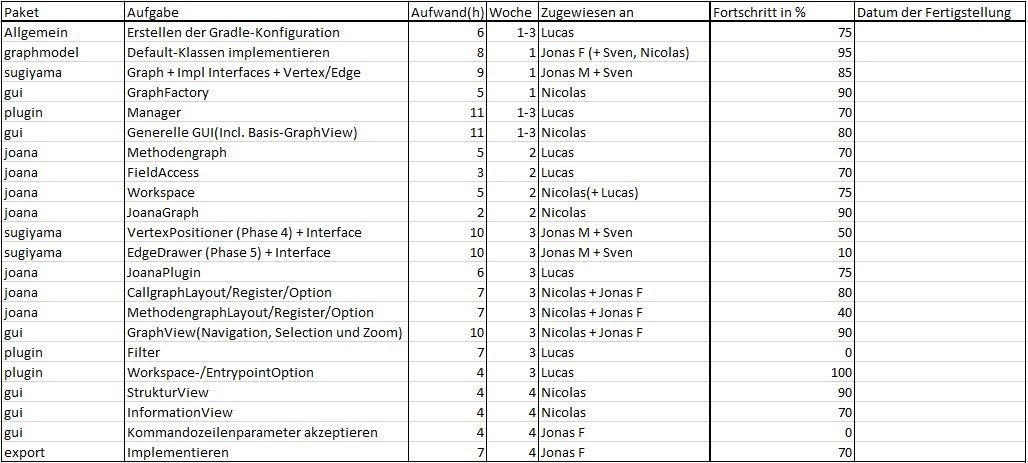
\includegraphics[width=380pt]{week_three_table.PNG}
	\caption{Implementierungsplan nach Woche 3}
	\label{fig:week_three_table}
\end{figure}
\subsection{Verzögerungen}
Nach dem Sprint zum Ende der zweiten Woche wurde, wie in \ref{fig:week_three_diagram} zu sehen ist, zunächst weniger gearbeitet. Ab Mitte der Woche wurde aber wieder der normale Arbeitsrythmus aufgenommen und es kam zu keinen weiteren Verzögerungen.
\begin{figure}[!htbp]
	\centering
	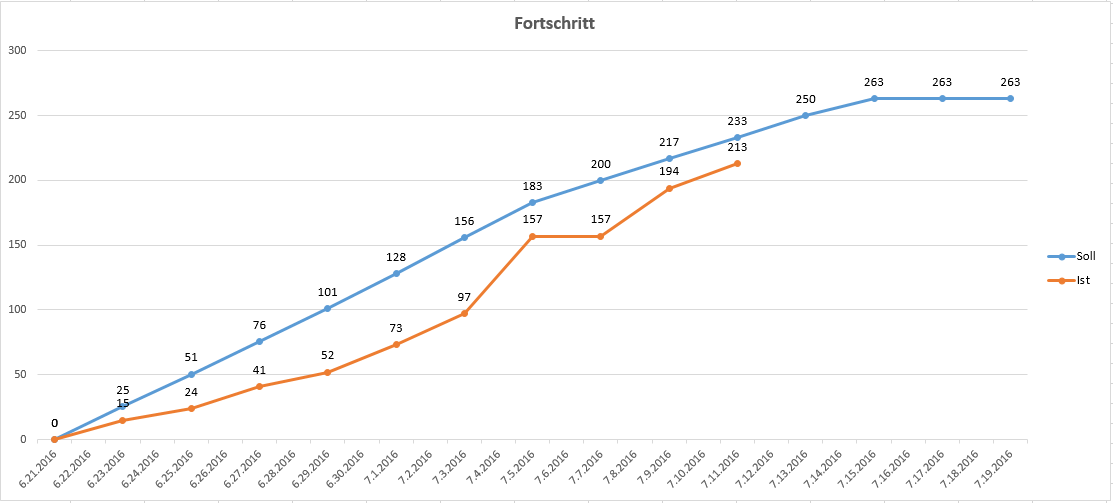
\includegraphics[width=380pt]{resourcen/week_three_diagram.PNG}
	\caption{Fortschrittsdiagramm nach Woche 3}
	\label{fig:week_three_diagram}
\end{figure}

\newpage

\section{Woche 4}
In Woche 4 wurden die vielen in Woche 3 begonnenen Aufgaben fertiggestellt. Des weiteren wurden Aufgaben die noch nicht begonnen waren, wie Filter und Kommandozeilenparameter akzeptieren, schnellstmöglich eingebaut.
Die Arbeit an den Filtern und dem Sugiyama-Algorithmus zog sich bis zum letzten Tag vor Fertigstellungstermin.
\subsection{Verzögerungen}
Die vielen weit fortgeschrittenen Aufgaben in Woche 3 die bereits in der Oberfläche benutzbar waren, zeigten verschiedene kleinere Fehler auf, die zuvor nicht sichtbar waren. Diese Fehler zu reparieren und die Tatsache das die Arbeit am Implementierungsheft begonnen wurde, sorgte für leichte Verzögerungen im Implementierungsfortschritt.
\begin{figure}[!htbp]
	\centering
	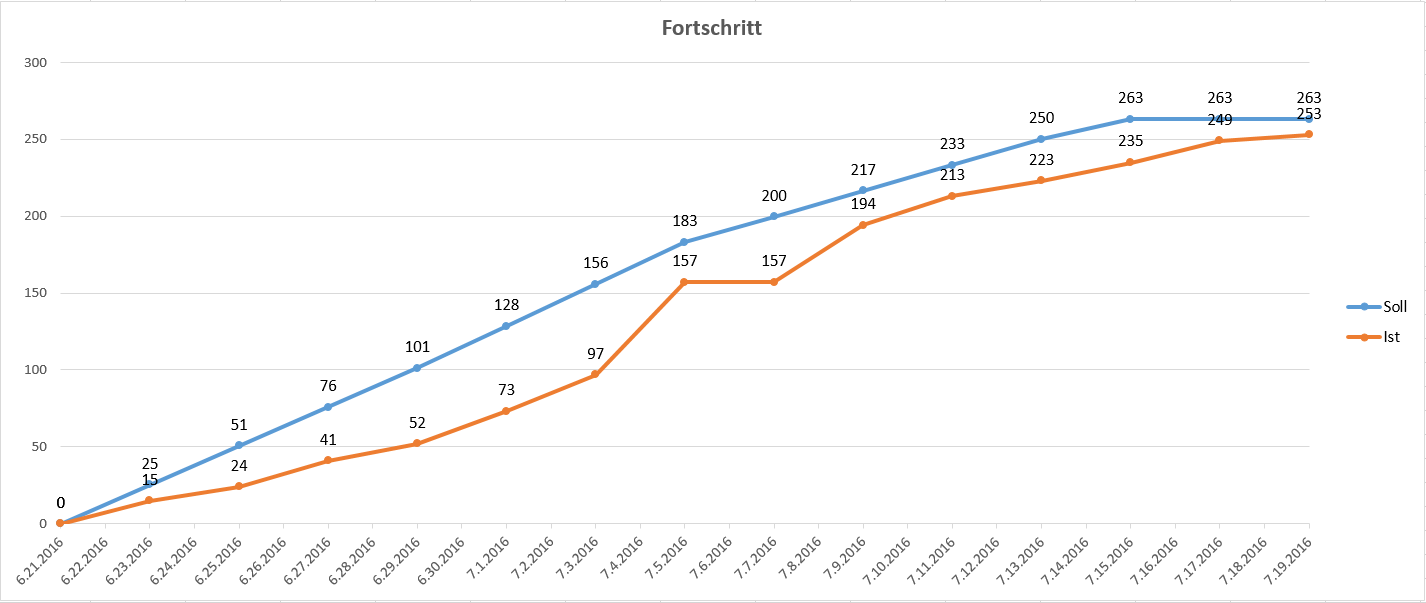
\includegraphics[width=380pt]{resourcen/week_four_diagram.PNG}
	\caption{Fortschrittsdiagramm nach Woche 4}
	\label{fig:week_four_diagram}
\end{figure}

\section{Rückblick}
Am Ende der 4. Woche steht rückblickend fest, dass der Implementierungsplan zwar von seiner Struktur und den generellen zeitlichen Abschätzungen gut war, der Arbeitsaufwand aber in vielen Aufgabenbereichen stark unterschätzt wurde. Der Grund war häufig, das im Entwurf gemachte Designentscheidungen nicht tief genug durchdacht waren und im Laufe der Entwicklung angepasst oder komplett neu erdacht werden mussten. Solche Anpassungen haben an verschiedenen Stellen sehr viel Zeit in Anspruch genommen, welche nicht im Implementierungsplan vermerkt wurde. Diese Verzögerungen spiegeln sich besonders in der flachen Fortschrittskurve in den ersten zwei Wochen dar und haben die gesamte Entwicklung zurückgeworfen. \\
Man erkennt in \ref{fig:week_four_diagram} das die Ist-Kurve nach der ersten Woche fast genau so stark, manchmal sogar stärker, steigt als die Soll-Kurve. Trotzdem wurde durch die nötigen Anpassungen bedeutend mehr Zeit gebraucht als angegeben wurde. Deshalb waren auch die 16 wöchentlichen Arbeitsstunden pro Person, mit welchen die Soll-Kurve berechnet wurde, bei weitem nicht ausreichend um die Entwicklung in den vier Wochen möglichst vollständig abzuschließen. Es wurden auch die fünf Tage am Ende, die als zeitlicher Puffer eingeplant waren vollständig benötigt.